% !TEX root = main.tex

\subsection{Analyzing Data Dependencies}


\begin{frame}{Next optimization!}
Before we got sidetracked by the loop unrolling stuff, LLVM-MCA told us there was a \alert{data dependency} bottleneck
\begin{block}{Bottleneck View}
\txtinput[\tt\fontsize{5.7pt}{6pt}\selectfont]{listings/01_add_reduction_v1_p04.txt}
\end{block}
\end{frame}


\begin{frame}{Next optimization!}
The problem is that every sum we perform depends on the result of the previous one.
\bigskip
\begin{block}{Data Dependency Graph}
\begin{center}
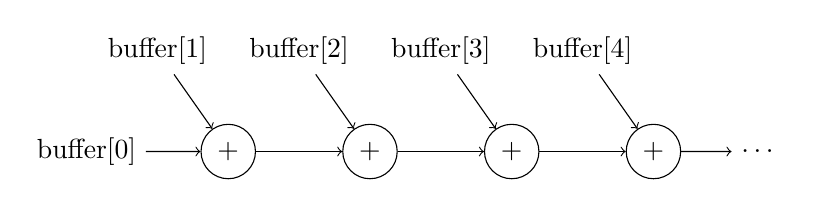
\begin{tikzpicture}[
		xscale=.9,yscale=0.64,
		inp/.style = {->},
		operation/.style = {circle, draw}
	]
	\node (b0) at (1,1) {buffer[0]};
	\node (b1) at (2,3) {buffer[1]};
	\node (b2) at (4,3) {buffer[2]};
	\node (b3) at (6,3) {buffer[3]};
	\node (b4) at (8,3) {buffer[4]};
	\node (sum0) [operation] at (3,1) {$+$};
	\node (sum1) [operation] at (5,1) {$+$};
	\node (sum2) [operation] at (7,1) {$+$};
	\node (sum3) [operation] at (9,1) {$+$};
	\node (dots) at (10.5,1) {\ldots};
	
	\path [inp] (b0) edge (sum0);
	\path [inp] (b1) edge (sum0);
	\path [inp] (b2) edge (sum1);
	\path [inp] (sum0) edge (sum1);
	\path [inp] (b3) edge (sum2);
	\path [inp] (sum1) edge (sum2);
	\path [inp] (b4) edge (sum3);
	\path [inp] (sum2) edge (sum3);
	\path [inp] (sum3) edge (dots);
\end{tikzpicture}

\medskip
\[
\textsf{result} = \left(\left(\left(\textsf{buffer[0]} + \textsf{buffer[1]}\right) + \textsf{buffer[2]}\right) + \textsf{buffer[3]}\right) + \ldots
\]
\end{center}
\end{block}
\end{frame}


\begin{frame}{Next optimization!}
If we exploit the associativity of addition, we can shorten the depth of our dependency chain!
\medskip
\begin{block}{Data Dependency Graph}
\small
\begin{center}
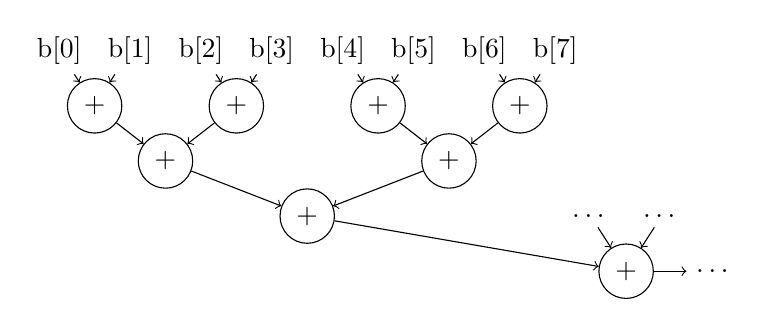
\begin{tikzpicture}[
		xscale=.45,yscale=0.7,
		inp/.style = {->},
		operation/.style = {circle, draw}
	]
	\node (b0) at ( 0,4) {b[0]};
	\node (b1) at ( 2,4) {b[1]};
	\node (b2) at ( 4,4) {b[2]};
	\node (b3) at ( 6,4) {b[3]};
	\node (b4) at ( 8,4) {b[4]};
	\node (b5) at (10,4) {b[5]};
	\node (b6) at (12,4) {b[6]};
	\node (b7) at (14,4) {b[7]};
	\node (sumL0I0) [operation] at (1,3) {$+$};
	\node (sumL0I1) [operation] at (5,3) {$+$};
	\node (sumL0I2) [operation] at (9,3) {$+$};
	\node (sumL0I3) [operation] at (13,3) {$+$};
	\node (sumL1I0) [operation] at (3,2) {$+$};
	\node (sumL1I1) [operation] at (11,2) {$+$};
	\node (sumL2I0) [operation] at (7,1) {$+$};
	\node (sumNext) [operation] at (16,0) {$+$};
	\node (dotsNextL1I0) at (15,1) {\ldots};
	\node (dotsNextL1I1) at (17,1) {\ldots};
	\node (dotsNextNext) at (18.5,0) {\ldots};
	
	\path [inp] (b0) edge (sumL0I0);
	\path [inp] (b1) edge (sumL0I0);
	\path [inp] (b2) edge (sumL0I1);
	\path [inp] (b3) edge (sumL0I1);
	\path [inp] (b4) edge (sumL0I2);
	\path [inp] (b5) edge (sumL0I2);
	\path [inp] (b6) edge (sumL0I3);
	\path [inp] (b7) edge (sumL0I3);
	\path [inp] (sumL0I0) edge (sumL1I0);
	\path [inp] (sumL0I1) edge (sumL1I0);
	\path [inp] (sumL0I2) edge (sumL1I1);
	\path [inp] (sumL0I3) edge (sumL1I1);
	\path [inp] (sumL1I0) edge (sumL2I0);
	\path [inp] (sumL1I1) edge (sumL2I0);
	\path [inp] (sumL2I0) edge (sumNext);
	\path [inp] (dotsNextL1I0) edge (sumNext);
	\path [inp] (dotsNextL1I1) edge (sumNext);
	\path [inp] (sumNext) edge (dotsNextNext);
\end{tikzpicture}

\end{center}
\[
\textsf{result} = \left(\left(\textsf{b[0]} + \textsf{b[1]}\right) + \left(\textsf{b[2]} + \textsf{b[3]}\right)\right) + \left(\left(\textsf{b[4]} + \textsf{b[5]}\right) + \left(\textsf{b[6]} + \textsf{b[7]}\right)\right) + \ldots
\]
\end{block}
\end{frame}


\begin{frame}{Next optimization!}
\begin{block}{Sum Reduction With Less Dependencies}
\cinput{listings/01_add_reduction_v3.c}
\end{block}
\end{frame}


\begin{frame}{Next optimization!}
\begin{columns}[onlytextwidth]

\column{0.7\textwidth}
\begin{block}{Sum Reduction With Less Dependencies}
\asminput[\tt\footnotesize]{listings/01_add_reduction_v3.s}
\end{block}

\column{0.25\textwidth}
\centering
LLVM is already helping the CPU scheduler by moving the access to \texttt{buffer[i+2]} before the access to \texttt{buffer[i+1]}!

\end{columns}
\end{frame}


\begin{frame}{What LLVM-MCA says...}
\begin{columns}

\column{0.45\textwidth}
\begin{block}{Before}
\asminput[\tt\small]{listings/01_add_reduction_v2_p01.txt}
\end{block}

\column{0.45\textwidth}
\begin{block}{After}
\asminput[\tt\small]{listings/01_add_reduction_v3_p01.txt}
\end{block}

\end{columns}
\medskip
The amount of work per iteration has stayed the same, and the cycle count is massively reduced!
\smallskip
From these figures, we expect the computation to complete in just $\approx\SI{0.01}{\second}$
instead than $\approx\SI{0.1}{\second}$!
\end{frame}


\begin{frame}{What the reality of facts says}
\begin{block}{Let's run it!}
\txtinput[\tt\small]{listings/01_add_reduction_v2_vs_v3_spdup.txt}
\end{block}
\medskip
\begin{description}[Good:]
\item[Good:] There is a huge improvement indeed!
\item[Bad:] The improvement is \alert{much less} than what we expected.
\end{description}
\end{frame}


\begin{frame}{The impact of memory accesses}
\begin{columns}

\column{0.55\textwidth}
\begin{block}{add\_reduction\_v3\_nocache.c}
\cinput[\tt\scriptsize]{listings/01_add_reduction_v3_nocache.c}
\end{block}
\begin{block}{Execution Time}
\txtinput[\tt\scriptsize]{listings/01_add_reduction_v3_nocache_spdup.txt}
\end{block}

\column{0.45\textwidth}
\begin{itemize}
\item Experiment: let's reduce the impact of memory accesses as much as possible
\item LLVM-MCA's analysis is the same even for the modified program
\item The real execution time now matches LLVM-MCA's prediction!
\end{itemize}

\end{columns}
\end{frame}


\begin{frame}{The impact of memory accesses}
\large
\begin{itemize}
\item Memory accesses are \alert{really slow}
\item Once the code is reasonably optimized, it will spend \alert{more time waiting for data to arrive} than performing actual calculations
\bigskip
\normalsize
\item This doesn't mean that, when it reaches that stage, the code cannot be optimized further.
\item Simply, any improvement from now on will be \alert{marginal}, especially for an algorithm like this one where there is not much we can do to improve memory access patterns.
\bigskip
\footnotesize
\item To solve the problem of memory access cost, some computer scientists have theorized computing systems where many small CPUs are embedded inside memory chips (\cite{MUTLU201928}).
\end{itemize}
\end{frame}


\begin{frame}{What can we do}
\begin{block}{Bottleneck View}
\txtinput[\tt\small]{listings/01_add_reduction_v3_p04.txt}
\end{block}
\begin{itemize}
\item We no longer have memory dependencies
\item Now it seems that we have excessive resource pressure
	\begin{itemize}
	\item \texttt{SKLPort2} and \texttt{SKLPort3} are used by \alert{load instructions}
	\item It seems we are issuing more loads than the CPU can perform 
	\end{itemize}
\end{itemize}
\end{frame}


\begin{frame}{What can we do}
\begin{itemize}
\item Let's scale back the ratio between memory accesses and add instructions a little bit...
\item Note that we are actually \alert{lengthening} the chain of data dependencies by doing this!
\end{itemize}

\begin{block}{Sum Reduction V3b}
\cinput{listings/01_add_reduction_v3b.c}
\end{block}
\end{frame}


\begin{frame}{Results}
\begin{block}{Sum Reduction V3b}
\txtinput{listings/01_add_reduction_v3_vs_v3b_spdup.txt}
\end{block}
\begin{itemize}
\item The tradeoff was worthwhile! We squeezed out some residual speedup from the code.
\end{itemize}
\end{frame}


\begin{frame}{In conclusion...}
We just made a piece of code \alert{worse} wrt. data dependencies... and there was a speedup!
\smallskip
\large
\begin{itemize}
\item You must always strike the right balance between different contrasting behaviors
	\begin{itemize}
	\item Data dependencies vs. resource usage
	\item Loop overhead vs. code cache and branch prediction
	\item Memory access patterns vs. algorithmic complexity
	\end{itemize}
\smallskip
\item You cannot reach the highest possible computation speed without machine-specific optimizations
	\begin{itemize}
	\item On a CPU architecture with more than 2 load ports, the situation is reversed and the code with 4 additions per cycle is now slower
	\end{itemize}
\end{itemize}
\end{frame}




